% Pour faire une référence d'une annexe
% (Annexe \ref{sec:nomsection} page~\pageref{sec:nomsection})

\section{Un peu d'histoire : exemple de texte neumé}
\label{sec:exempleTexteNeume}
\begin{figure}[!htbp]
	\centering
	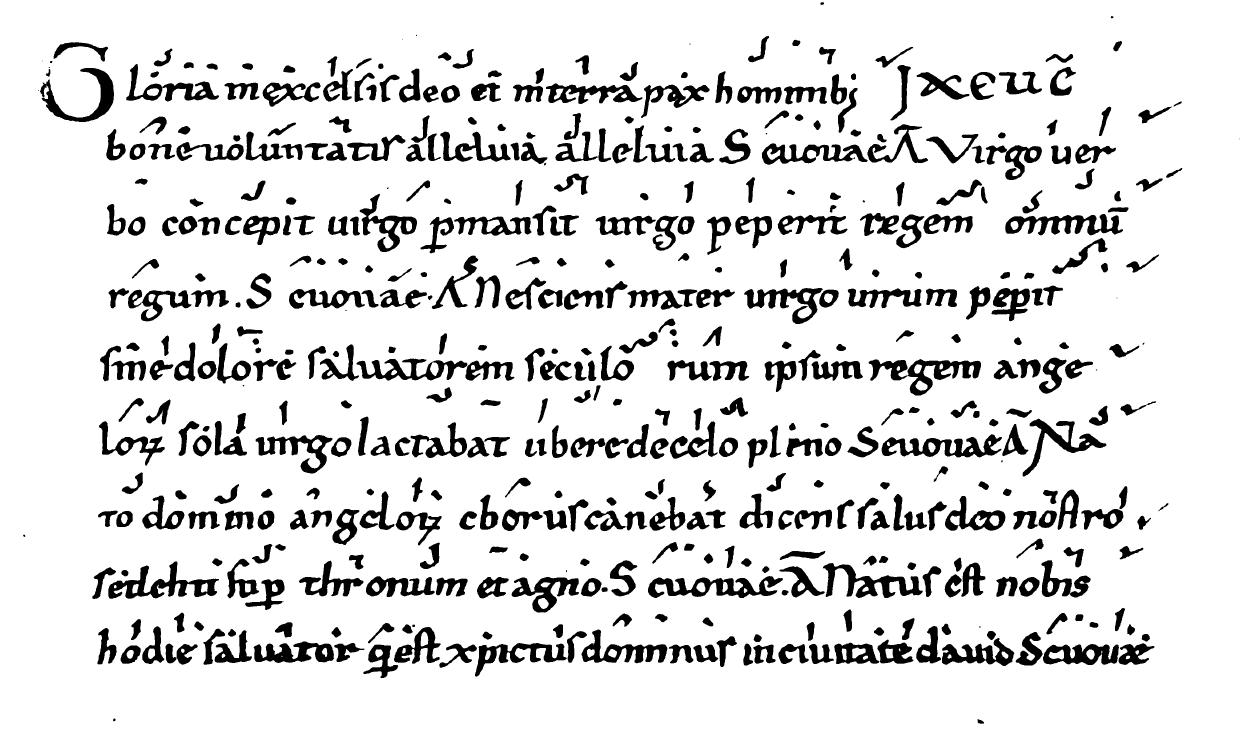
\includegraphics[keepaspectratio=true, width=\textwidth]{Annexes/i/neumes.jpg}
	\caption{Exemple de texte neumé  }
	\medskip
	\small	
	Source : 1774, Martin Gerbert, \textit{De cantu et musica sacra a prima Ecclesiae aetate usque ad praesens Tempus}, St. Blasien, Typis San-Blasianis, t. I, t. II. - \textit{Les neumes sont les symboles inscrient au-dessus des mots du chant liturgique (ici le chant} Gloria \textit{de l'ordinaire de la messe).}
	\label{fig:neumes}
\end{figure}
\clearpage

\section{Un peu d'histoire : exemple de notation carrée}
\label{sec:exempleNotationCarree}
\begin{figure}[H]
	\centering
	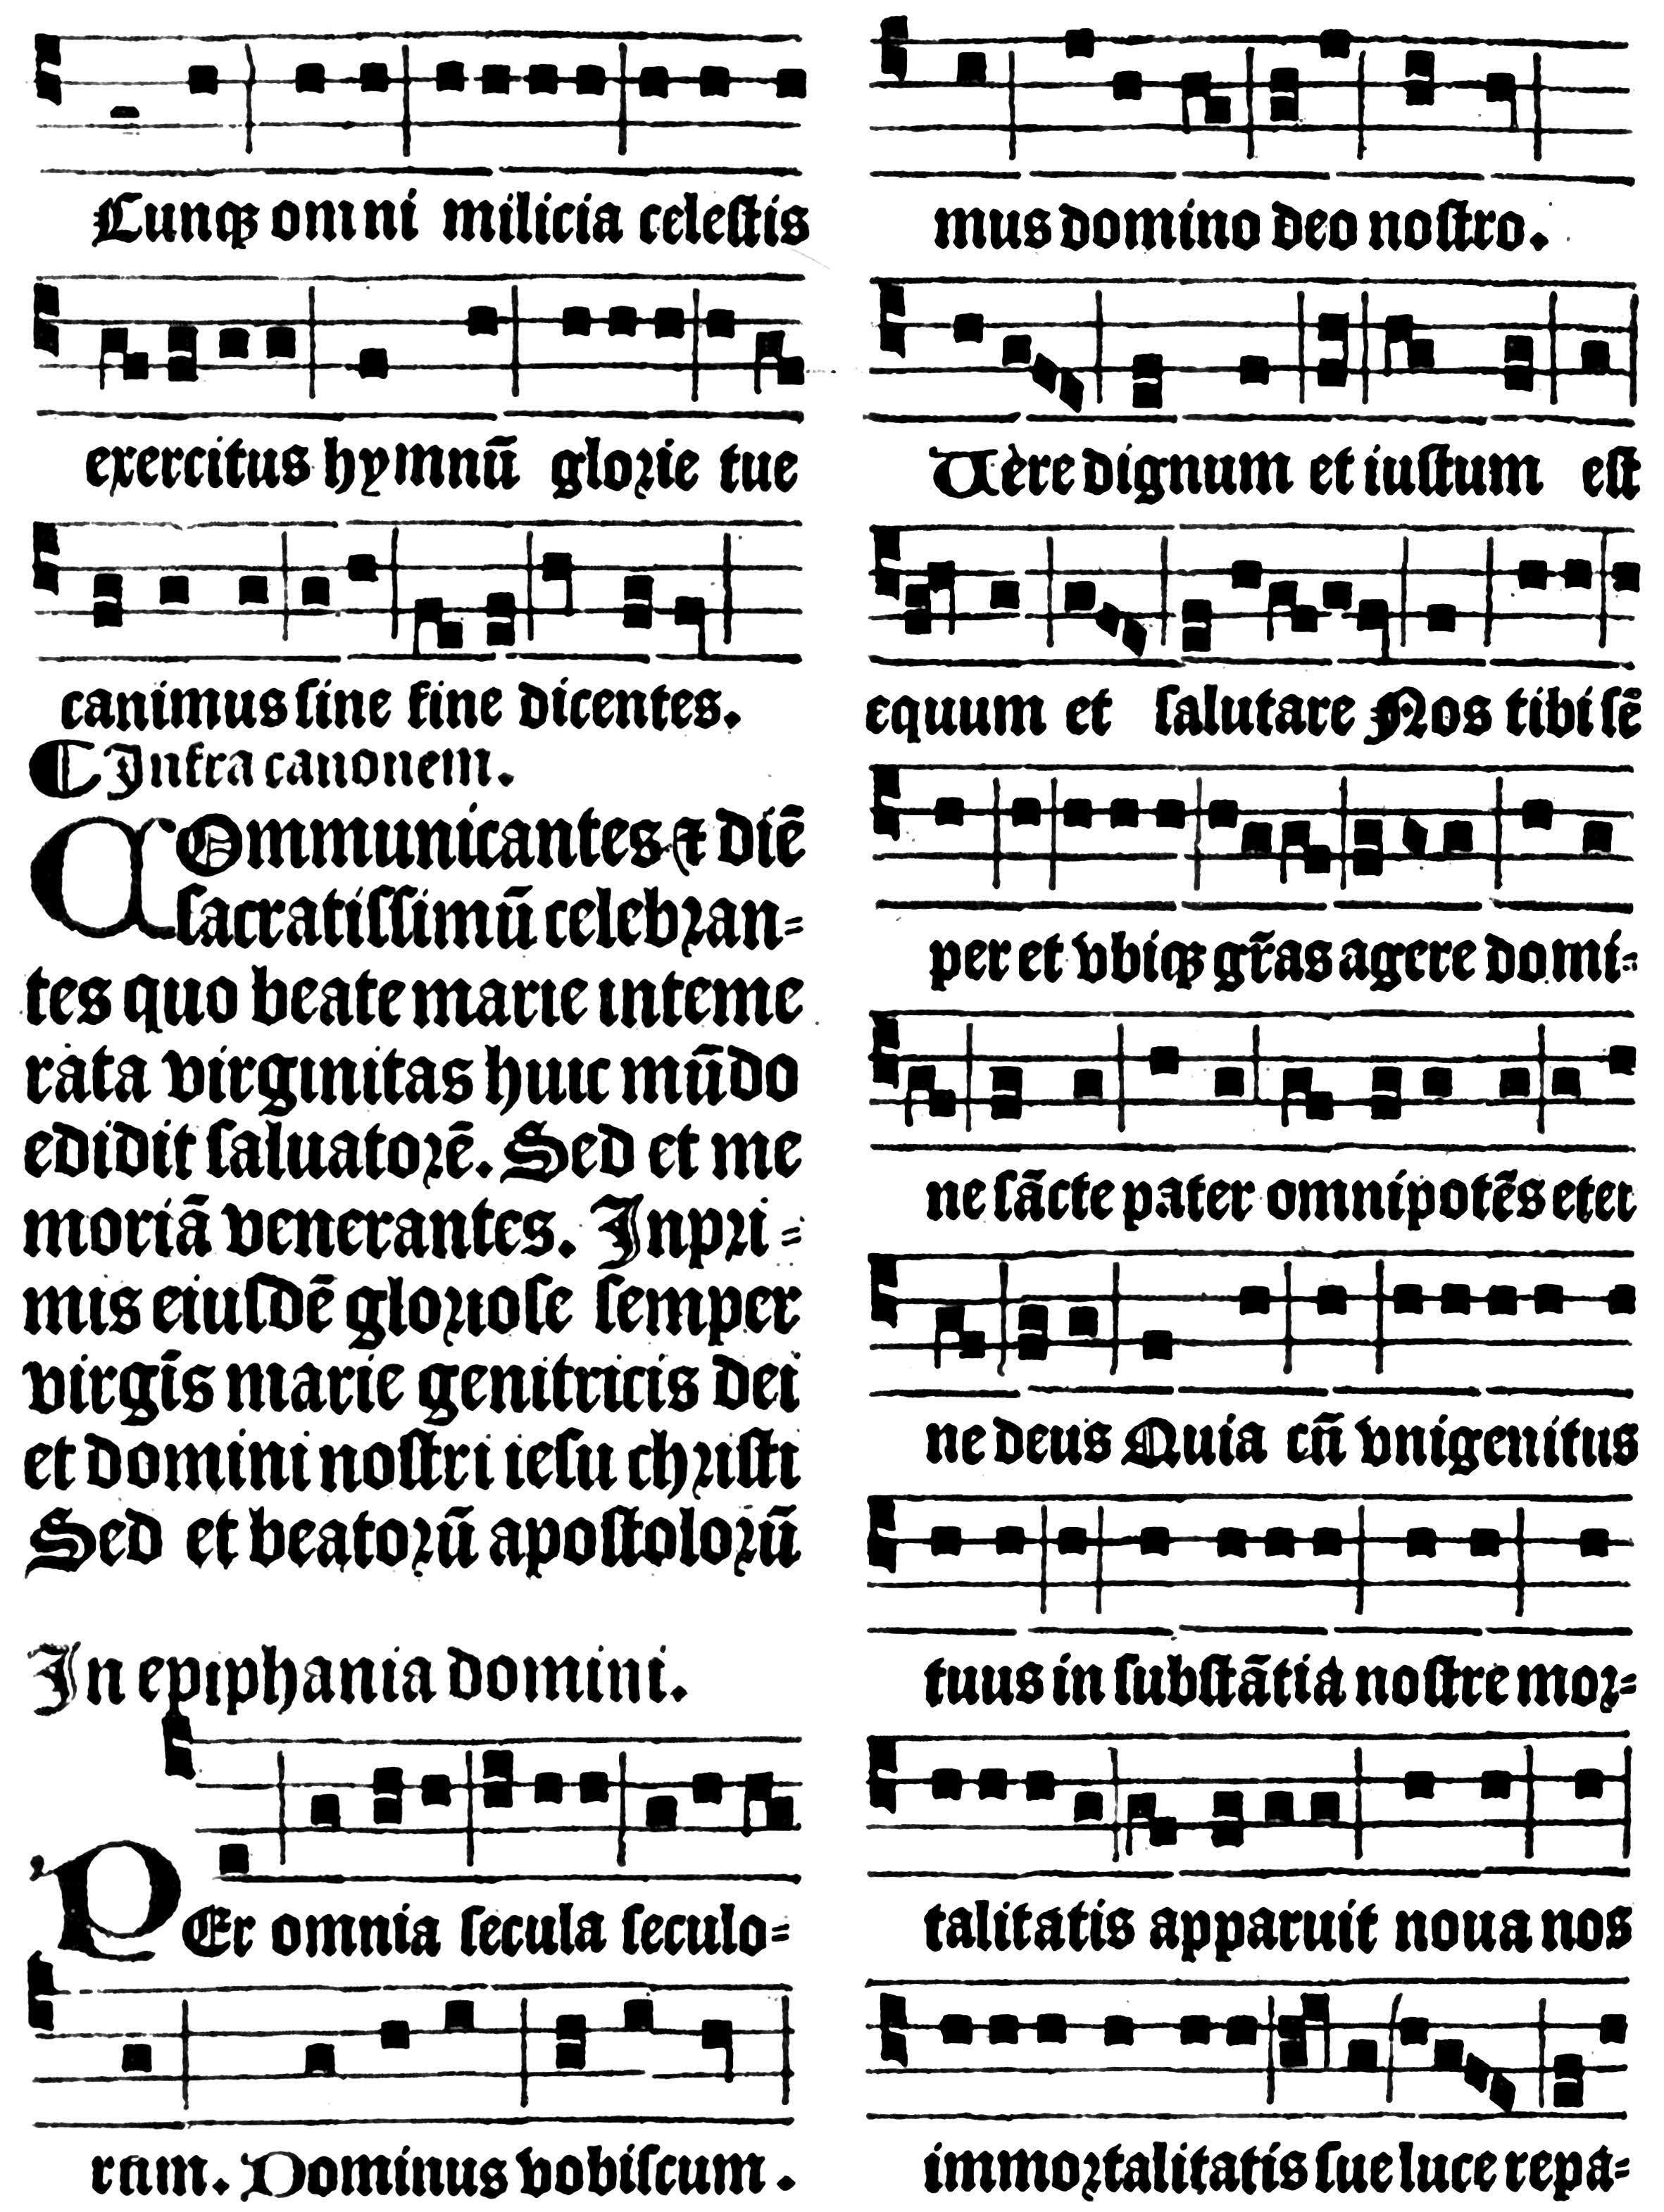
\includegraphics[keepaspectratio=true, width=\textwidth]{Annexes/i/notationCarree.jpg}
	\caption{Exemple de notation carrée "imprimée"}
	\medskip
	\small
	Source : 1499, Jean Highman, \textit{Missale Leodiense}, Paris - \textit{Les notes sont représentées en notation carrée toujours au-dessus du texte chanté.}
	\label{fig:notationCarree}
\end{figure}
\clearpage

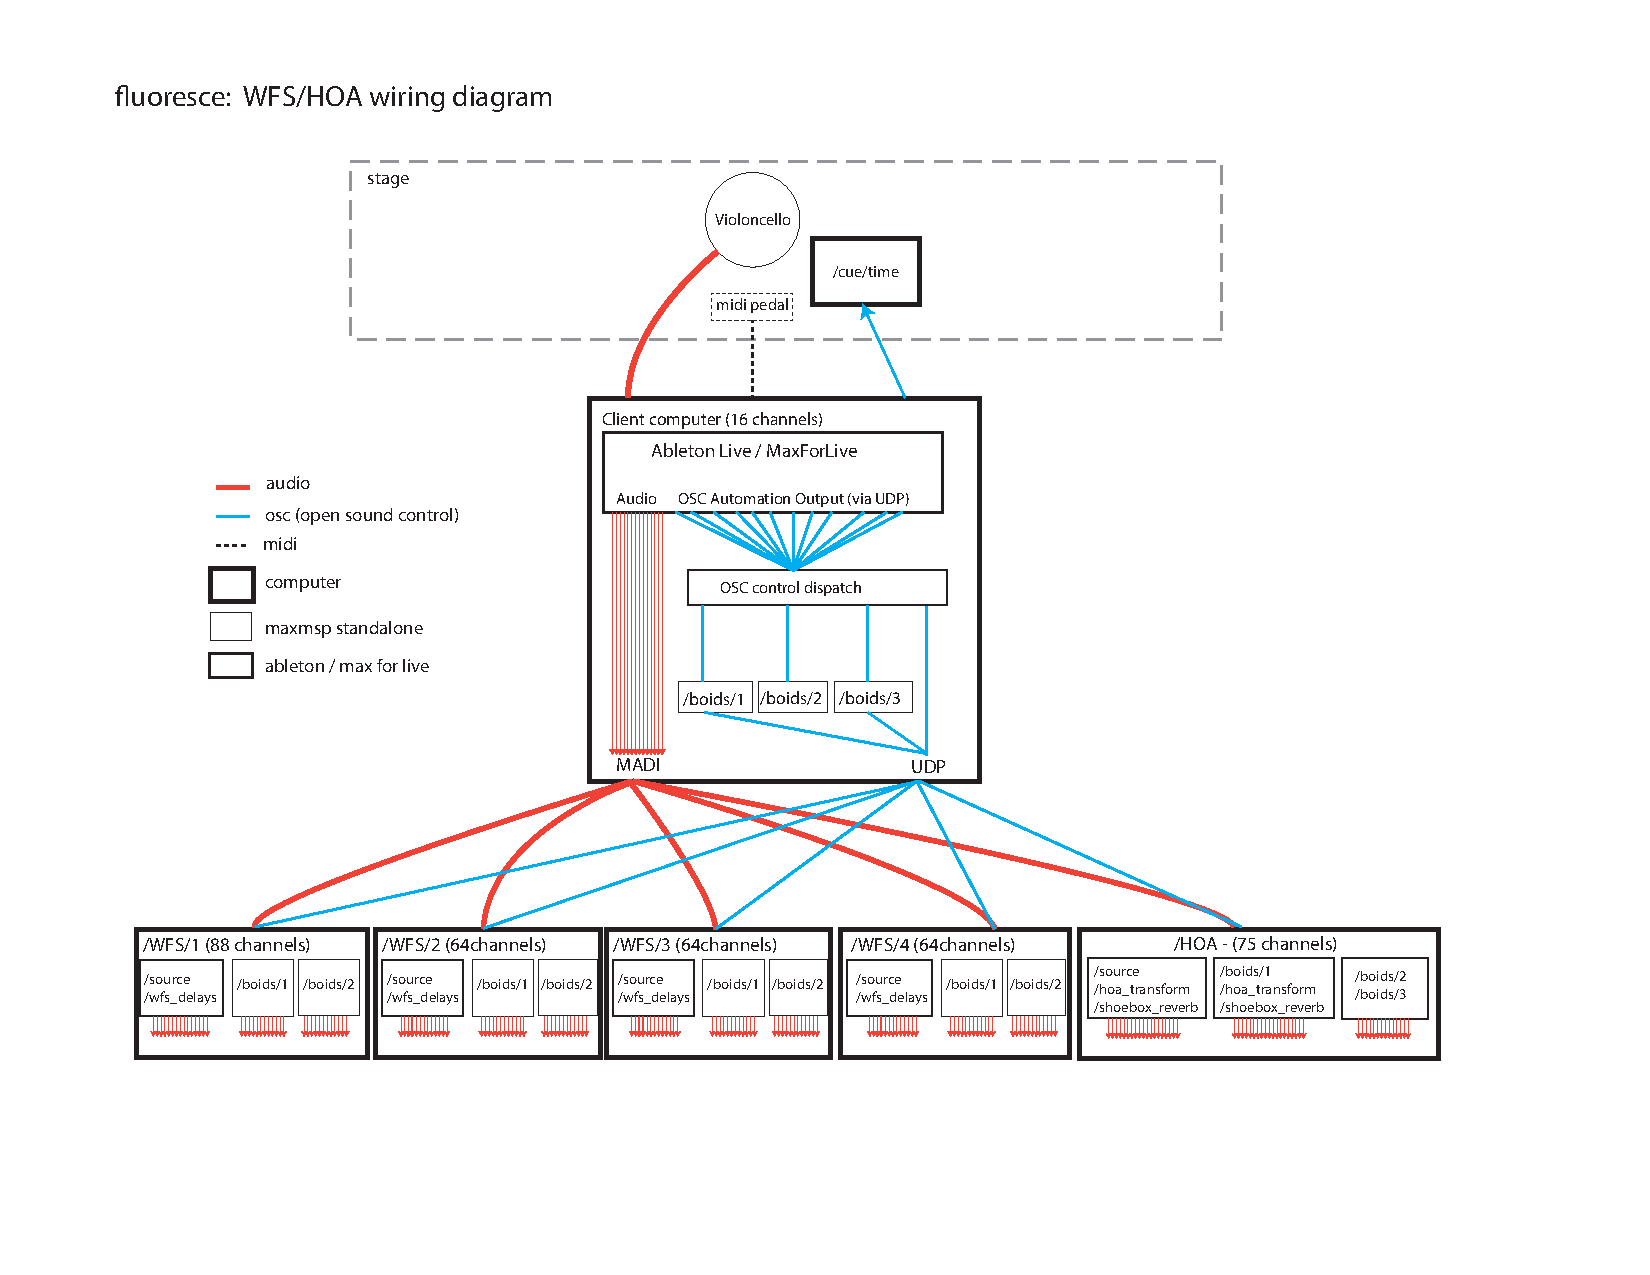
\includepdf[
	angle = 90,
	addtolist={1, figure, {Schéma complet de branchement pour la pièce \textit{Fluoresce}, Rama Gottfried, 2012}, fig:schemaInstallationFluoresceComplet}, 
	pagecommand = {
		\section{Noter la musique multimédia : schéma complet de branchement pour la pièce \textit{Fluoresce}, Rama Gottfried, 2012}
		\label{sec:schemaInstallationFluoresceComplet}
	}]{Annexes/schemaInstallationFluoresceComplet.pdf}

\section{Noter la musique multimédia : deux transcriptions de la pièce \textit{Reflets de l'ombre}, Carmine E. Cella, 2013}
\label{sec:refletsDeLOmbre}

\begin{figure}[!htbp]
	\centering
	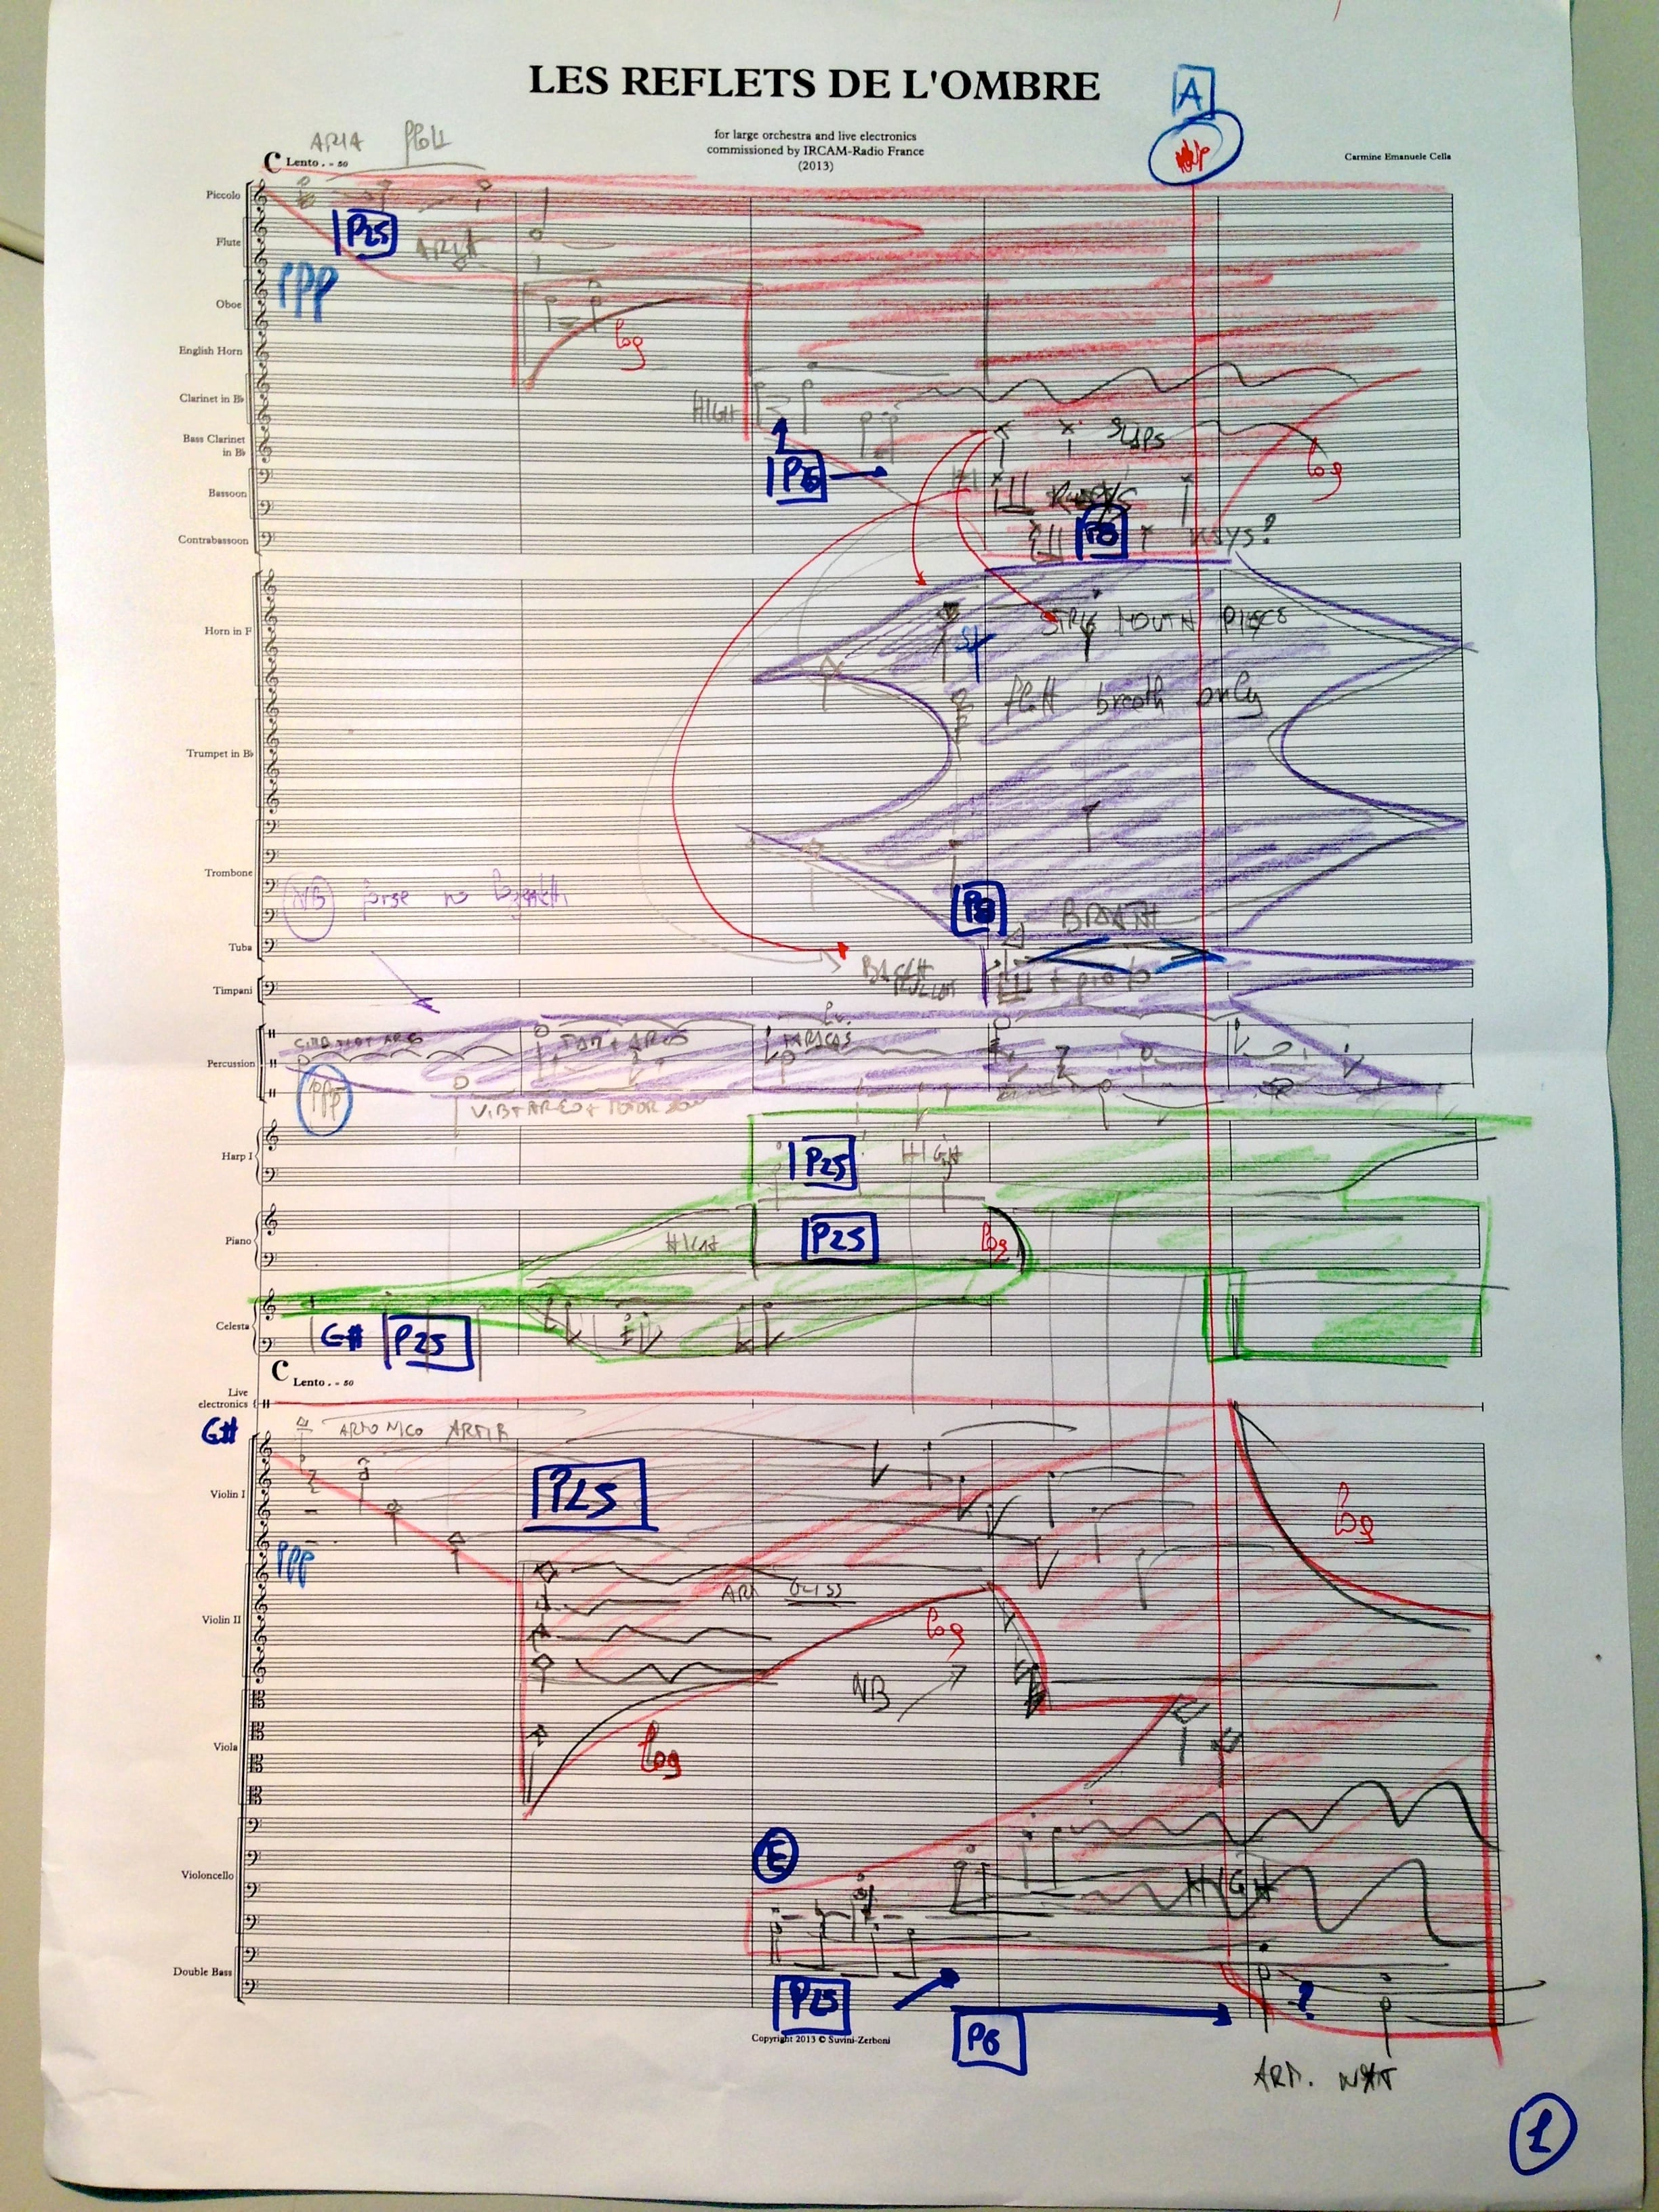
\includegraphics[keepaspectratio=true, width=\textwidth, angle = -90]{Annexes/i/refletsDeLOmbreFantaisie.jpg}
	\caption{Extrait d'une première version de \textit{Reflets de l'ombre} par Carmine E. Cella}
	\medskip
	\small
	\textit{Cette première version représente la pièce en termes de variations du timbre du son.
	La musique y est notée de manière quasi morphologique, avec quelques ajouts de symboles de la gravure standard.}	
	\label{fig:refletsDeLOmbreFantaisie}
\end{figure}

\begin{figure}[!htbp]
	\centering
	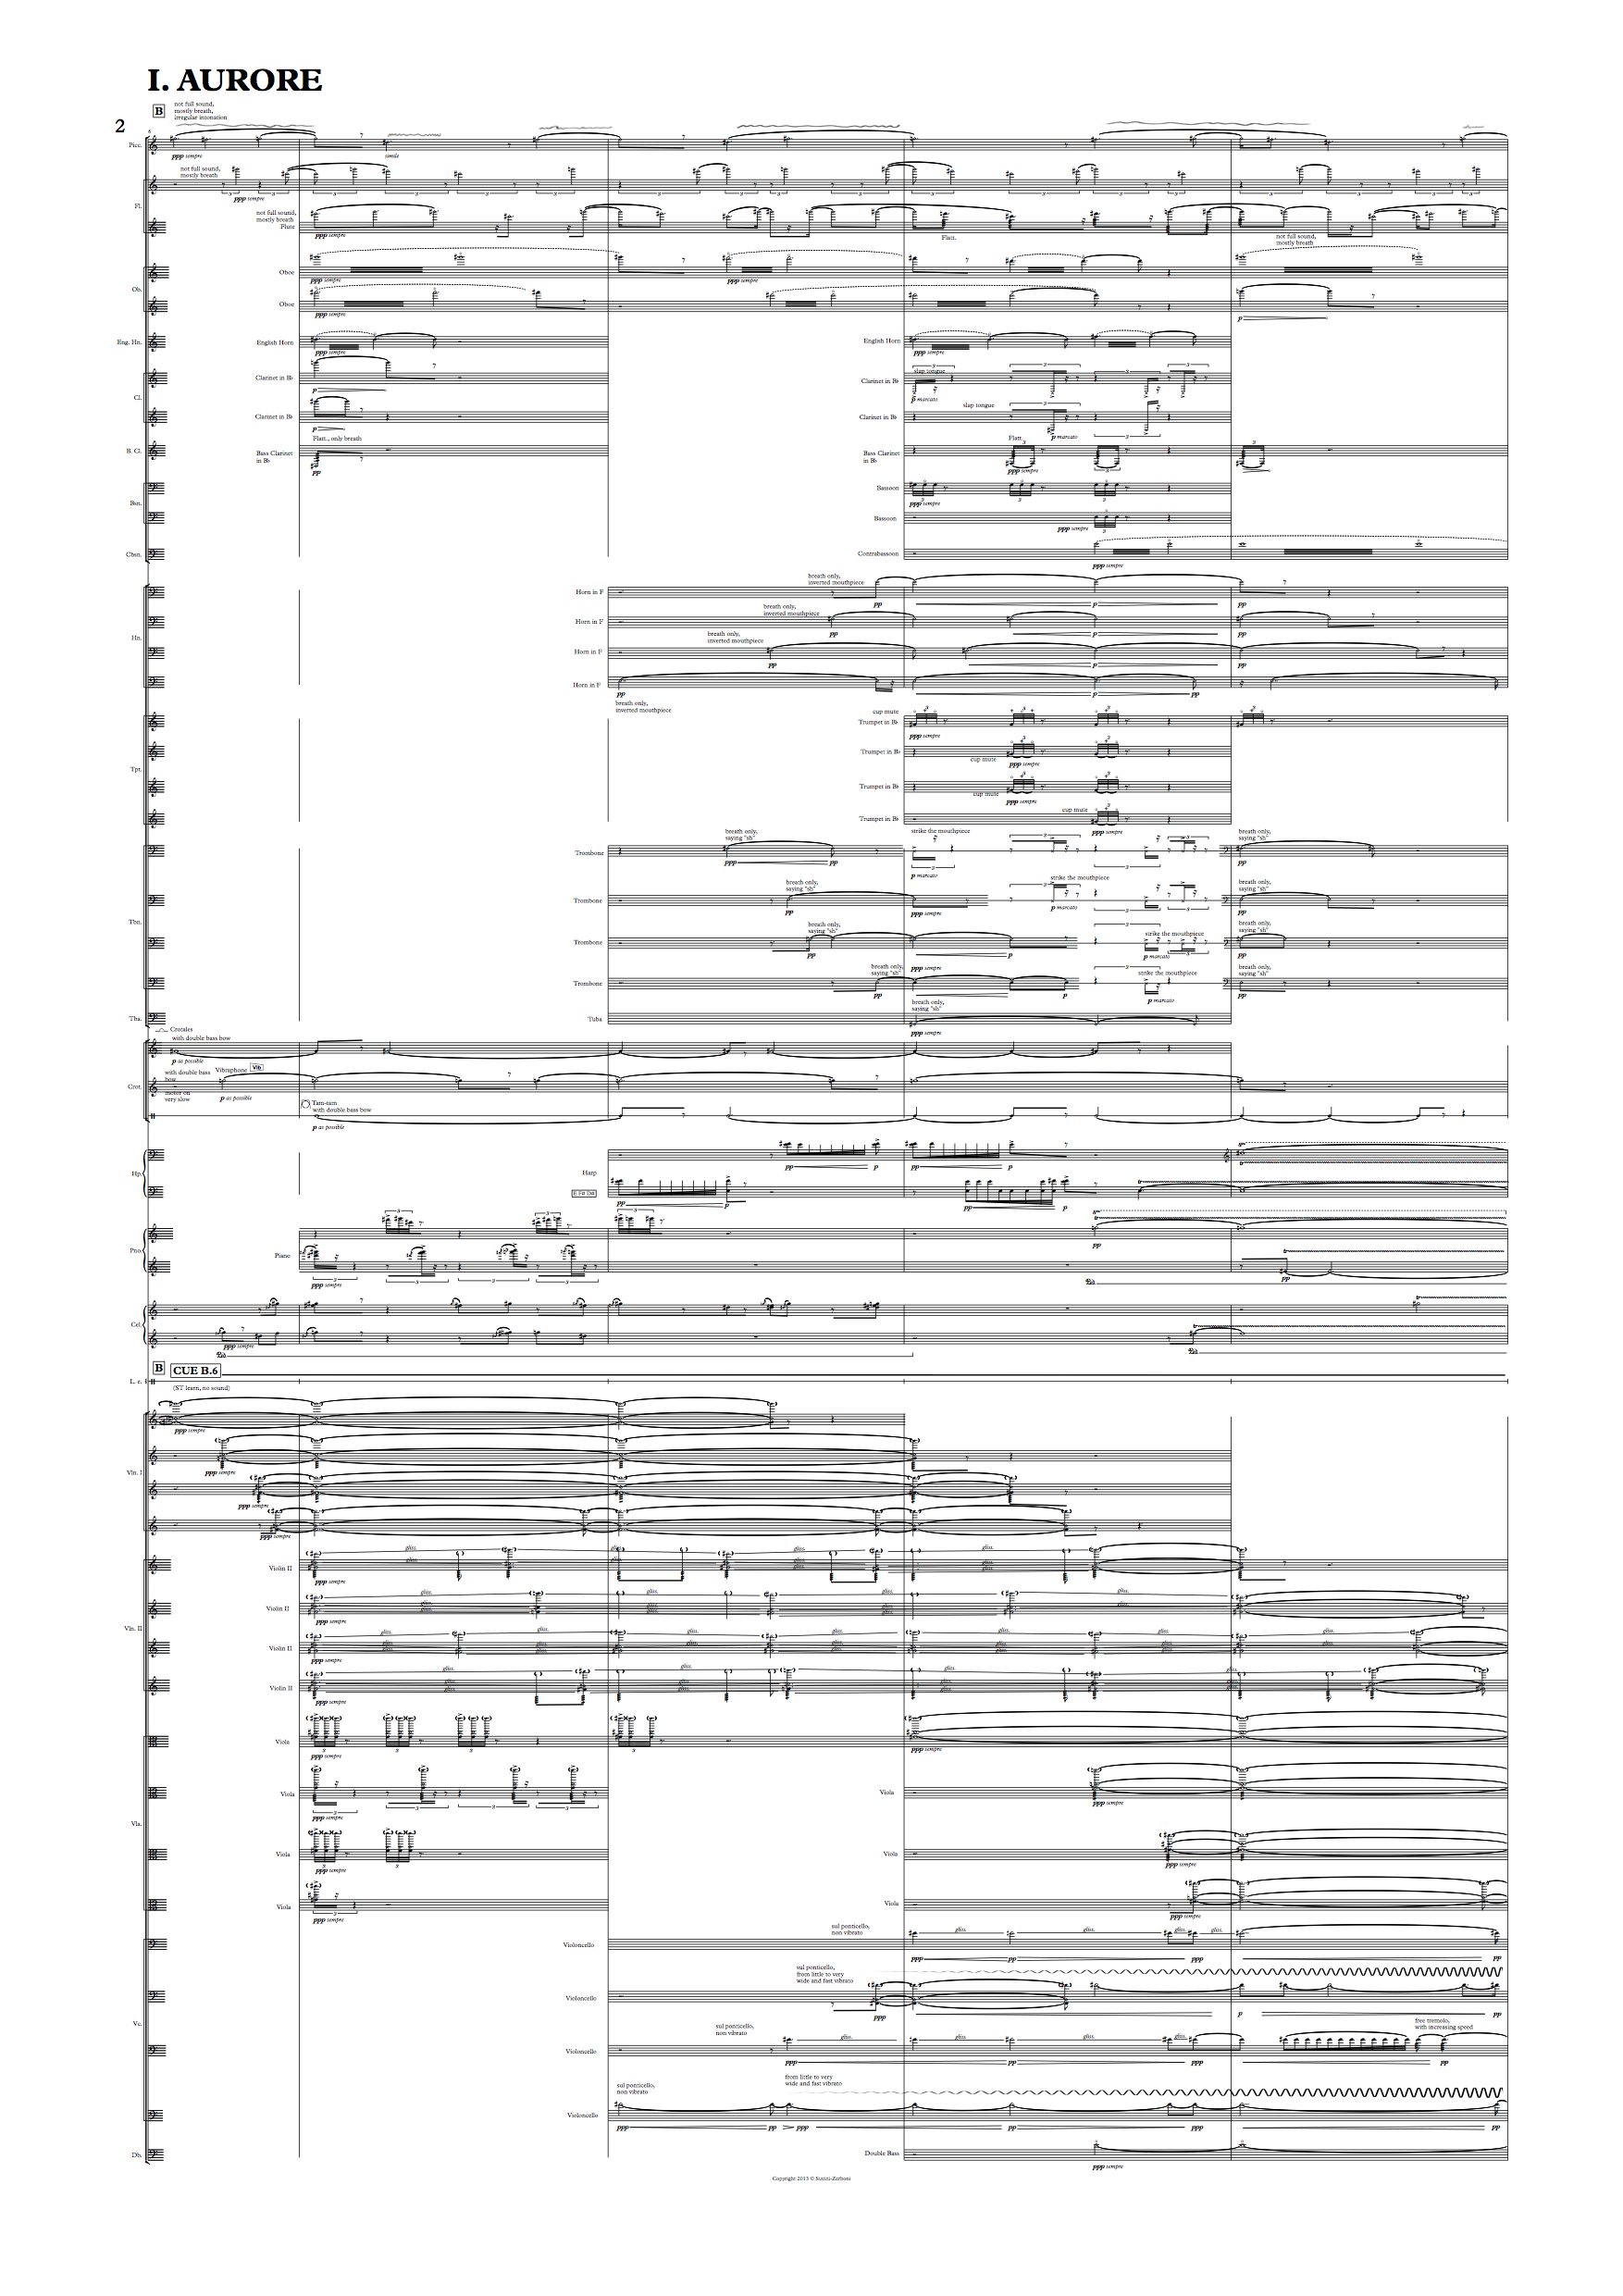
\includegraphics[keepaspectratio=true, width=\textwidth]{Annexes/i/refletsDeLOmbreReel.png}
	\caption{Extrait d'une version éxecutée par un orchestre de \textit{Reflets de l'ombre} par Carmine E. Cella}
	\medskip
	\small
	Cette version de la pièce, qui est destinée à l'orchestre exécutant, a été remaniée vis à vis de la version de la figure \ref{fig:refletsDeLOmbreFantaisie}. Cependant, les formes du son se retrouvent même dans cette transcription plus littérale. 	
	\label{fig:refletsDeLOmbreReel}
\end{figure}
